\section{Amplificador operacional y lista de materiales}
\label{sec:ao}

\subsection{Datos de hoja técnica}
En el laboratorio hay TL081, TL084, TL071, TL072 y LM358. El TL072 disponible está marcado \textbf{TL072CP}: Texas Instruments, rango comercial
(\qtyrange{0}{70}{\degreeCelsius}) y encapsulado PDIP-8. La \cref{tab:ao} resume los parámetros relevantes según las hojas de datos de
TI~\cite{ti_tl07x,ti_lm358}. La revisión actual de la hoja TL07xx especifica un GBW típico de \qty{5.25}{\mega\hertz} para este encapsulado, mientras
que las revisiones anteriores (y la versión de ST~\cite{st_tl072}) indican entre \qty{3}{\mega\hertz} y \qty{4}{\mega\hertz}. Para no depender de la
revisión del silicio, los cálculos usan \qty{3}{\mega\hertz}.

\begin{table}[H]
  \centering\footnotesize
  \caption{Parámetros de los AO disponibles ($V_{CC} = \qty{\pm 15}{\volt}$, \qty{25}{\degreeCelsius}).}
  \label{tab:ao}
  \tabres{tab_ao}
\end{table}

\subsection{Efecto del GBW finito}
Se repitió el análisis nodal reemplazando ambos AO por $A(s) = \omega_t/s$. La desviación de $\lvert H\rvert$ respecto del caso ideal
(\cref{fig:gbw}) es como máximo de \qty{\vGBWdevTL}{\decibel} hasta \qty{4}{\kilo\hertz} con el TL072CP (con \qty{3}{\mega\hertz}) y de
\qty{\vGBWdevLM}{\decibel} con el LM358. Con $f_0 \approx \qty{1.2}{\kilo\hertz}$ y ganancia unitaria, ambos AO tienen GBW de sobra.

\begin{figure}[H]
  \centering
  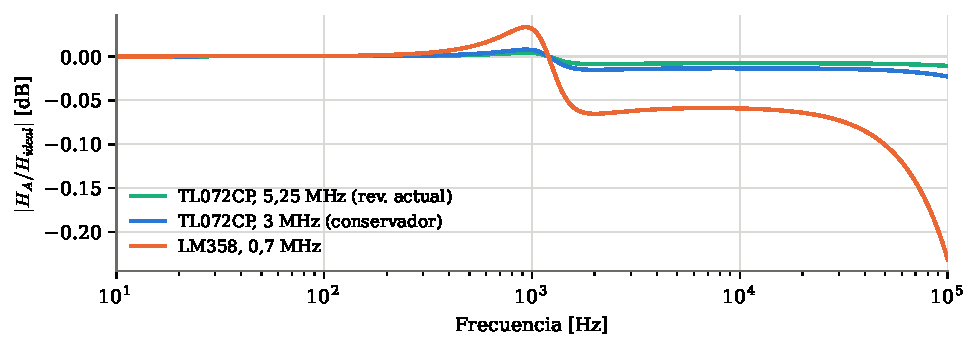
\includegraphics[width=0.85\linewidth]{fig_gbw_finito}
  \caption{Desviación de la respuesta por GBW finito (modelo de un polo), con los valores adoptados.}
  \label{fig:gbw}
\end{figure}

\subsection{Amplitud máxima, slew rate, modo común y carga}
\begin{itemize}
  \item \textbf{Niveles internos.} Con la cascada en el orden elegido, $\max\lvert V_2/V_i\rvert$ y $\max\lvert V_6/V_i\rvert$ valen 1 (en continua) y
        $\max\lvert V_4/V_i\rvert = \num{\vNodoCuatroMax}$ (en \qty{\vNodoCuatroF}{\hertz}). En régimen transitorio, el sobrepico de la respuesta
        al escalón es de \qty{\vSobrepico}{\percent}.
  \item \textbf{Excursión y modo común.} Con alimentación de \qty{\pm 12}{\volt} se adopta un margen de \qty{3}{\volt} a cada riel, que es el mínimo
        de hoja de datos para $R_L = \qty{10}{\kilo\ohm}$. Ese margen cubre también el límite inferior del modo común de la familia TL07x, que no
        llega al riel negativo. Resulta $\lvert v\rvert \le \qty{9}{\volt}$ en todo nodo, y por lo tanto $V_{i,p} \le \qty{\vVinMax}{\volt}$.
  \item \textbf{Slew rate.} Con una entrada senoidal de \qty{\vVinMax}{\volt} de pico en la peor frecuencia, la pendiente máxima es de
        \qty{\vSRUuno}{\volt\per\micro\second} en U1 y de \qty{\vSRUdos}{\volt\per\micro\second} en U2. Ante un escalón de la misma amplitud es de
        \qty{\vSREscalon}{\volt\per\micro\second}. Todos estos valores quedan más de dos órdenes de magnitud por debajo del mínimo garantizado de
        \qty{8}{\volt\per\micro\second}.
  \item \textbf{Carga.} U1 ve como mínimo la impedancia de entrada del Sallen--Key (\qty{\vZminUuno}{\kilo\ohm}); U2, su red de realimentación a
        través de $C_1$ (al menos \qty{\vZminUdos}{\kilo\ohm}) en paralelo con la carga externa del osciloscopio (\qty{1}{\mega\ohm}). Ambas superan
        los \qty{2}{\kilo\ohm} para los que la hoja de datos garantiza la excursión.
\end{itemize}

\subsection{Elección}
Se usa el \textbf{TL072CP} disponible, que aloja U1 y U2 en un solo encapsulado. Tiene entrada JFET con corrientes de polarización de pA
(irrelevantes con resistencias de decenas de k$\Omega$) y bajo ruido. Dos TL081 son un reemplazo directo, uno por etapa. El LM358 cumpliría en GBW y
slew rate para este filtro, pero se descarta por la distorsión de cruce de su etapa de salida, que no tiene polarización clase AB y trabajaría con
señal alterna centrada en \qty{0}{\volt}. También pesan su mayor corriente de polarización y ruido, y que su salida no llega a menos de
\qty{1.5}{\volt} del riel positivo.

Se alimenta con \qty{\pm 12}{\volt} desde la fuente partida del laboratorio, bien por debajo del máximo absoluto de \qty{\pm 18}{\volt}, con un
capacitor cerámico de \qty{100}{\nano\farad} junto a cada pin de alimentación y uno electrolítico de \qty{10}{\micro\farad} por riel. Para las
mediciones se propone una entrada de \qty{1}{\volt} eficaz (aprox. \qty{1.41}{\volt} de pico), con un margen de más de cinco veces respecto de la
saturación. Para medir la banda de rechazo con mejor relación señal/ruido se puede subir hasta unos \qty{5}{\volt} de pico.

\begin{table}[H]
  \centering\footnotesize
  \caption{Lista de materiales. En el filtro se usan capacitores de film (poliéster/MKT) o cerámicos C0G; se evitan los cerámicos de alta constante
  dieléctrica, cuyo valor varía con la tensión y la temperatura. Las resistencias indicadas con «+» se conectan en serie.}
  \label{tab:bom}
  \tabres{tab_bom}
\end{table}
